\documentclass[include/preamble.tex]{subfiles}
\begin{document}

\subsection{doof}

\begin{frame}[fragile]
  \begin{center}
    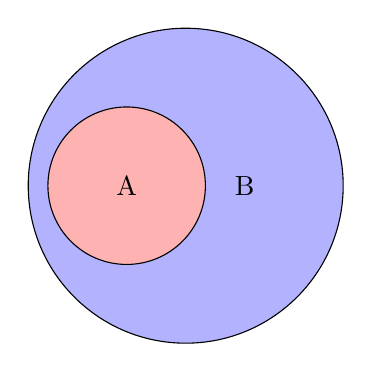
\begin{tikzpicture}
      \begin{scope}
        \draw[fill=blue!30!white] (0,0)     circle (2);
        \draw[fill=red!30!white]  (-0.75,0) circle (1);
      \end{scope}
      \node at (-0.75, 0)  {A};
      \node at ( 0.75, 0)  {B};
    \end{tikzpicture}
    \begin{tikzcd}[matrix scale=2.5]
      A
      \arrow[r, "\iota_{AB}"] &
      B \\
      Option[Int]
      \arrow[r, "\iota_{widen}"] &
      Iterable[int]
    \end{tikzcd}
    \begin{lstlisting}[style=scala]
      val a: Option[Int]   = Some(1)
      val b: Iterable[Int] = a
      val c: AnyRef        = b
    \end{lstlisting}
    \begin{tikzcd}[matrix scale=2.5]
      A
      \arrow[r, "\iota_{AB}"] &
      A + B \\
      Int
      \arrow[r, "\iota_{Left}"] &
      Either[Int, String]
    \end{tikzcd}
    \begin{lstlisting}[style=scala]
      val v: Either[Int, String] = Left(2)
    \end{lstlisting}
  \end{center}
\end{frame}

\begin{frame}[fragile]
  \begin{center}
    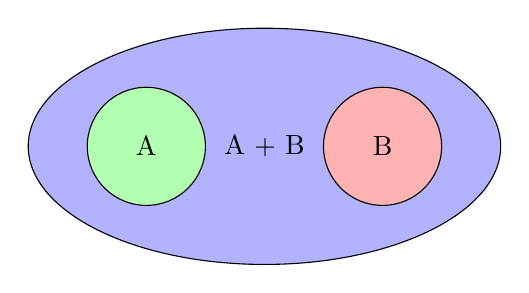
\begin{tikzpicture}
      \begin{scope}
        \draw[fill=blue!30!white]   (0,0) circle [x radius=3, y radius=1.5];
        \draw[fill=green!30!white] (-1.5,0) circle (0.75);
        \draw[fill=red!30!white]  (1.5,0)  circle (0.75);
      \end{scope}
      \node at (-1.5, 0)  {A};
      \node at ( 1.5, 0)  {B};
      \node at ( 0  , 0)  {A + B};
    \end{tikzpicture}
    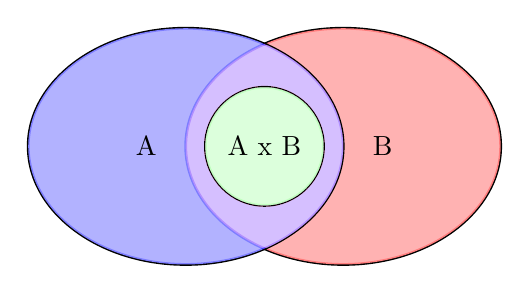
\begin{tikzpicture}
      \begin{scope}[blend group = soft light]
        \draw[fill=green!30!white] ( 0,0) circle (0.75);
        \draw[fill=blue!30!white]  (-1,0) circle [x radius=2, y radius=1.5];
        \draw[fill=red!30!white]   ( 1,0) circle [x radius=2, y radius=1.5];
      \end{scope}
      \node at (-1.5, 0)  {A};
      \node at ( 1.5, 0)  {B};
      \node at ( 0  , 0)  {A x B};
    \end{tikzpicture}
  \end{center}
\end{frame}

\end{document}
